\startchapter{Results}
\label{chapter:results}

In this section, I first describe my data preparation efforts.  
Next, I present models for locating the center of action and distinguishing left and right hand.  
Finally, I present some qualitative observations based on post-trial questions.
\begin{figure}[h]
 \centering
 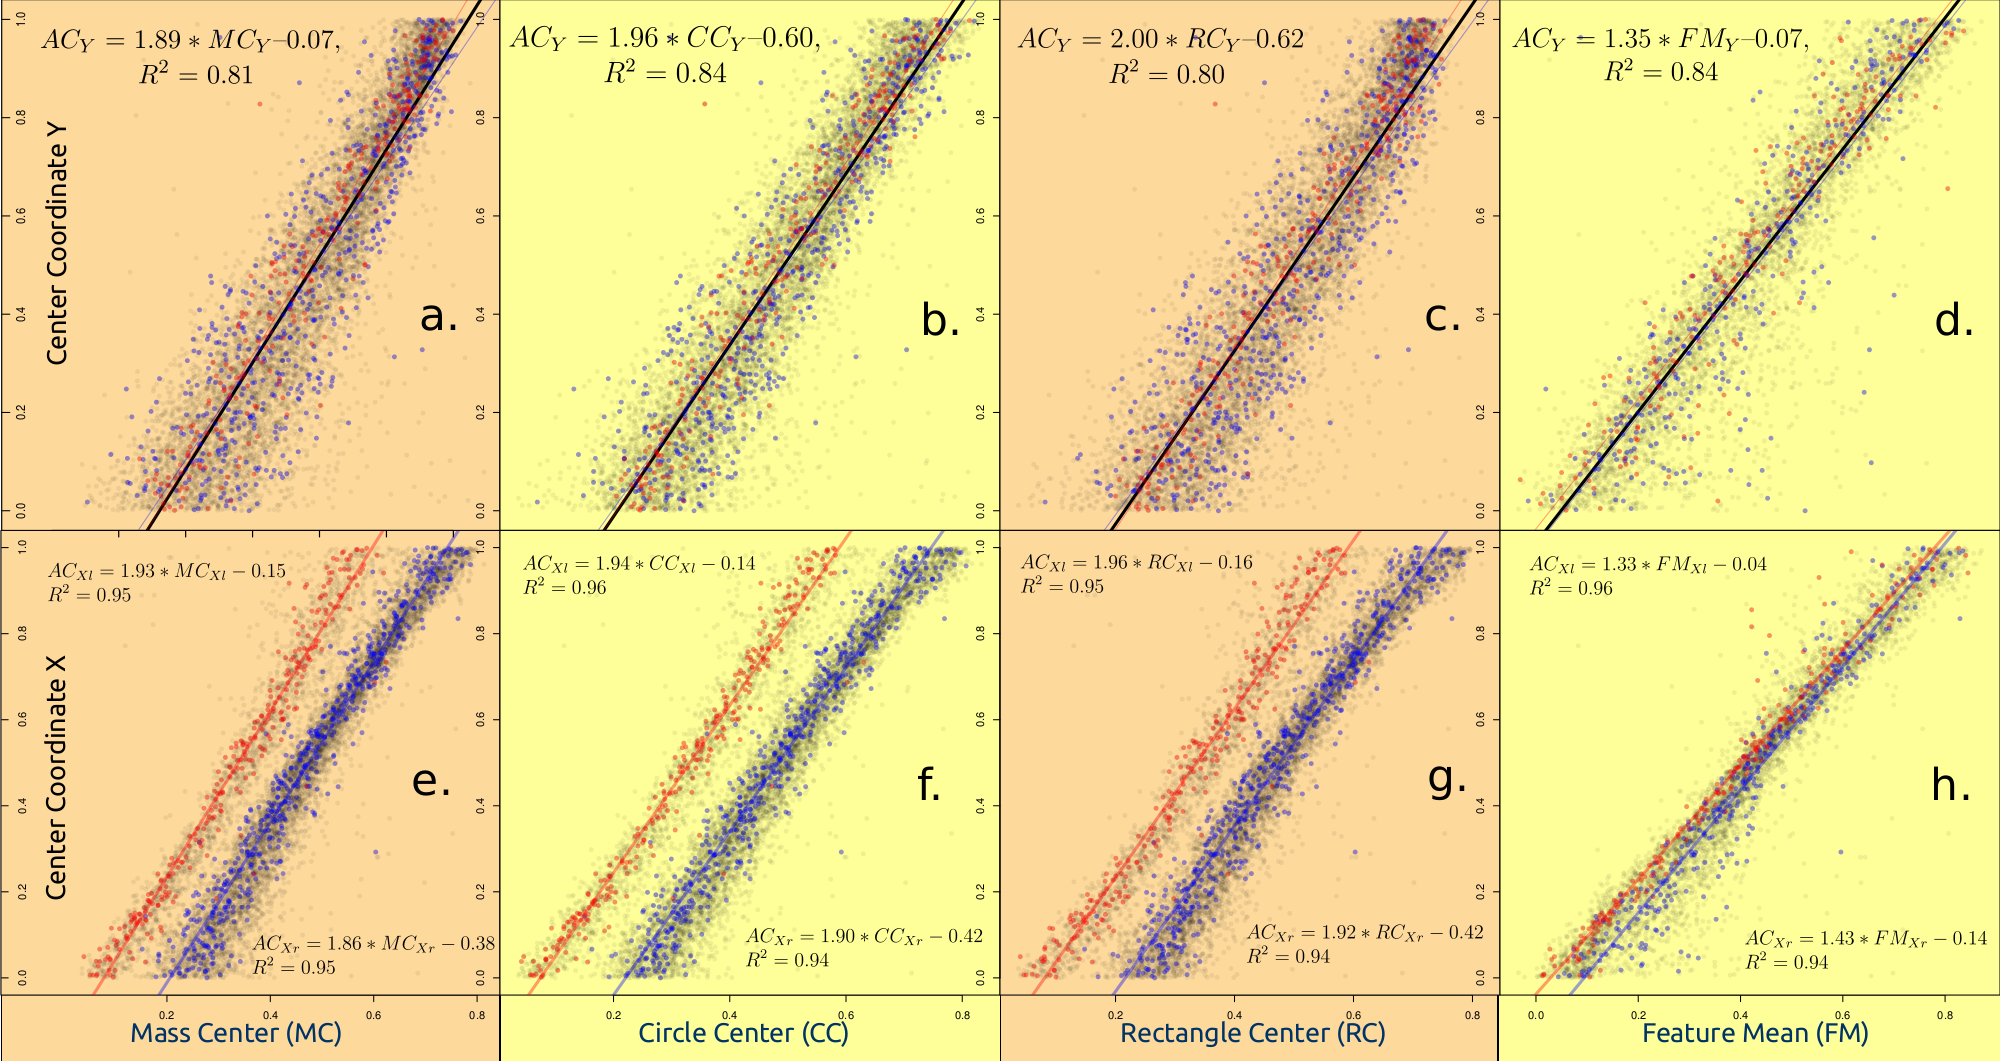
\includegraphics[width=6in]{./img/models_2x4.pdf}
 \caption{
Participant data of four models to predict X and Y coordinates of the center of action.
}
 \label{fig:models}
\end{figure}

\section{Data Preparation}
I filtered outliers and invalid records as follows.  
Data points outside the range $[quantile_1 - (1.5*IQR) , quantile_2 + (1.5 * IQR)]$ where IQR stands for Inter Quartile Range, were identified as outliers.  
%A total of ?? outliers (??\% of the data) were removed.
Records were invalid when they did not contain valid data from the tracking software; e.g., feature mean would be invalid when no features were identified by the optical flow tracking algorithm.

Mean values described in the following sections are based on an average of the last three video frames for a particular trial.  
In other words, I reduced the dimensionality of the multiple video frames per trial into a single representative value.  
Prior to this study, I did not know an appropriate temporal length for describing grab and release actions.  
I conducted informal pilots to estimate that 12 consecutive video frames would be a very conservative upper bound for all potential participants.  
I recorded 12 consecutive frames prior to registering each action for all study
trials.
The tracking software performed at a minimum of 7 FPS (Frames Per
Second) with both median and maximum rates of 9 FPS.  
Therefore, the length of temporal window in which the tracker collected its data was approximately 1.33 seconds.
I created correlation matrices from 12 video frames aggregated across all participants, and then visually identified frames that contained the highest correlation between predictors and response values - in my case X and Y positions of center of action.
Since the last three frames showed substantially higher correlations (above a threshold of 0.80), I reduced my data to contain only data from those three frames and thus reduced the length of the temporal window to 0.33 seconds. 
For each variable on each trial, I then take the mean value from those three frames.

\bigskip
\section{Model for Locating the Center of Action}
Center of action is the location on the 2D display where the user intends to center their grab or release interaction.
I investigate four potential models for identifying the center of grab and release actions.
Figure \ref{fig:models} captures a summary of the four linear regression models that I analyzed:  (MC) mass center, (CC) circle center, (RC) rectangle center, and (FM) feature mean.  
For the top row of Y coordinate data, the black line represents the linear regression over the whole dataset. 
Blue and red points represent the subsets of data that were identified to be performed by the right and left hands, respectively.
Hand side identification was performed by manually reviewing randomly selected sections of the study videos.
For the bottom row of X coordinate data, blue and red lines represent linear regressions over subsets of data that were identified to have been performed by right and left hands, respectively.  
All models are normalized plots of the Y and X coordinates for a hand shape model against the Y and X coordinates of the actual object or target.  
The Y and X coordinates were normalized by dividing them by height and width of the screen respectively to obtain a value between 0 and 1.
Plots a-d illustrate the unimodal distributions of data points for the Y coordinate results of each model, whereas plots e-h illustrate the bimodal distributions of data points for X coordinates, corresponding to the two hands.  
This result suggests that a system for detecting near touch actions needs to identify which hand is employed by the user.

\subsection{Effect of Hand Side}
I use analysis of covariance (ANCOVA) to compare left and right hand regression lines.
I analyze this effect only on the X coordinate because I observed a very small difference between the left and right hands along the vertical (Y coordinate) axis, which in my view is currently of little practical value.
However, the horizontal difference between the models is large, especially the distance between intercepts for left and right regression models.
For each of the four models, I consider the null hypothesis that there is no difference between regression lines for the left and the right hand.
Table 1 presents the ANCOVA results of hand side (HS) for each of the four models.

\begin{center}
\begin{table}
\centering
\caption[ANCOVA results of hand side for each of the four models:  Mean Center (MC), Circle Center (CC), Rectangle Center (RC), and Feature Mean (FM).]{ANCOVA results of hand side for each of the four models:  Mean Center (MC), Circle Center (CC), Rectangle Center (RC), and Feature Mean (FM).  
$\Delta{Slope}$ and $\Delta{Intercept}$ are the absolute value of the difference in slope and intercept, respectively, of the left and right hand data for each model.}
\rowcolors{2}{CornflowerBlue}{Dandelion}
\begin{tabular}{|l l l l l|}
\hline
\multicolumn{5}{|c|}{$H_0: Model_{right} = Model_{left}, \alpha = 0.01$}\\
Model  & F value & P value & $\Delta{Slope}$ & $\Delta{Intercept}$\\
\hline
$MC_X$& 6.8984 & 0.00878 & 0.07 & 0.23\\
$CC_X$& 12.355 & 0.00046 & 0.04 & 0.28\\
$RC_X$& 11.927 & 0.00058 & 0.01 & 0.26\\
$FM_X$& 16.649 & 5.158e-05 & 0.10 & 0.10\\
\hline
\end{tabular}
\end{table}
\end{center}
I observed statistically significant p-values to a level of $\textit{p} < .01$ in all four cases, so I can reject the null hypothesis in all four models. Thus, hand side is a significant variable for the X coordinate of a user's center of action.
Table 1 illustrates particularly large differences between left and right hand intercepts for the first three models MC, CC, and RC.  For the FM model, the slope is larger and intercept difference is smaller compared to the other three models.

\subsection{Effect of Object Size}
Object size was not observed to have a practical effect on the models and was not analyzed further.
\begin{figure}
\centering
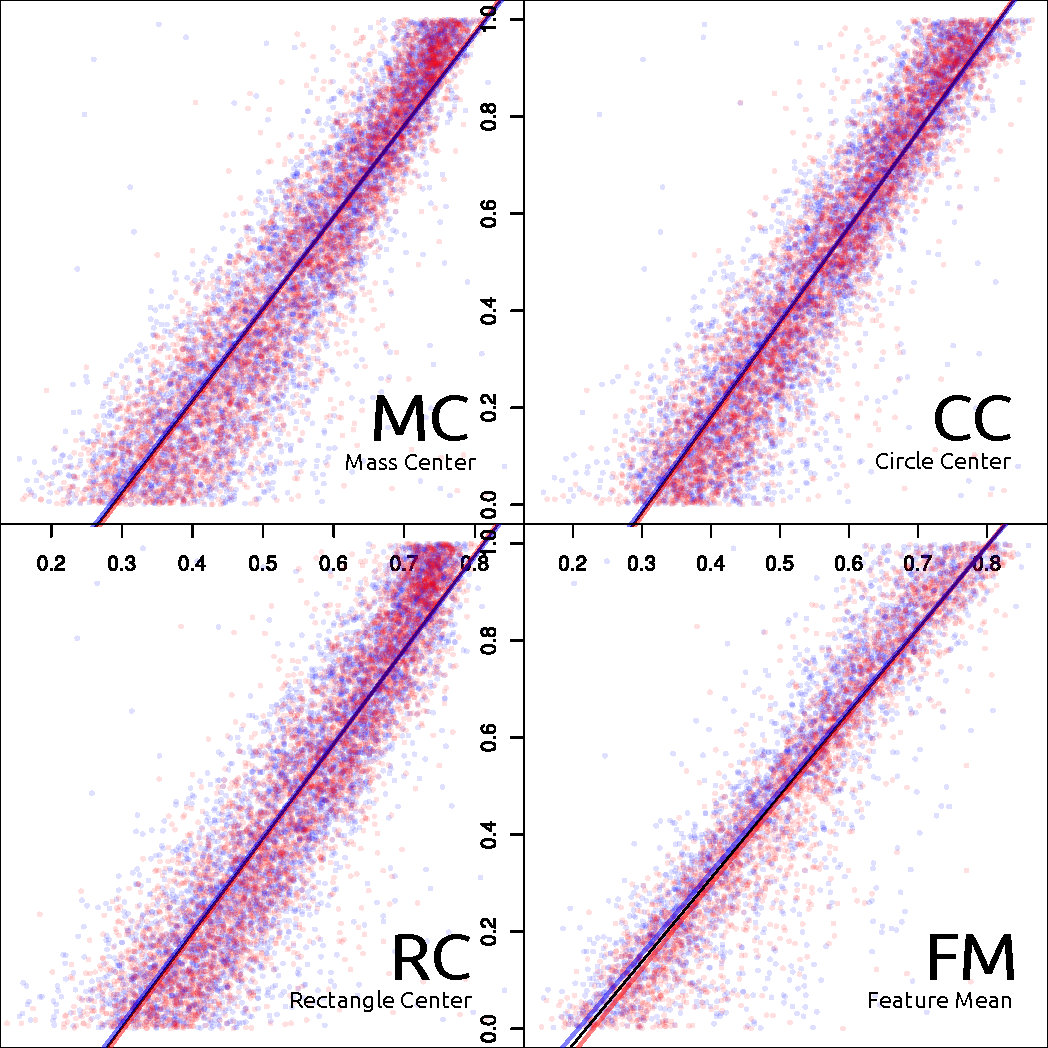
\includegraphics[type=pdf,ext=.pdf,read=.pdf,width=5in]{./img/Y_lm_actiontype_2x2}
\caption[Influence of action type on the regression models.]{
Influence of action type on the regression models. 
Red lines show the regression model only for the grab action, blue lines are for release action, and black lines are based on the whole dataset. 
}
\label{fig:Y_lm_actiontype}
\end{figure} 
\subsection{Effect of Action Type}
I also tested whether the type of action (grab versus release) performed by the user was a defining factor in determining the center of action.
Figure \ref{fig:Y_lm_actiontype} visualizes the alternative regression models considering the action type as a covariate factor for all four proposed models for center of action. As shown in the Figure, there is very little difference between the first three models, whereas the slope of the two regression lines are noticeably different for the feature mean (FM) model. 
For each of the four models in Figure \ref{fig:Y_lm_actiontype}, I consider the null hypothesis $H_0: Model_{grab} = Model_{release}, \alpha = 0.01$. 
Similar to effect of hand side, I use analysis of covariance (ANCOVA) to compare regression lines for grab and release actions.
\begin{center}
\begin{table}
\centering
\caption{Grab and release action type differences for the Y component of center of action}
\begin{tabular}{|l l l|}
\hline
\multicolumn{3}{|c|}{$H_0: Model_{grab} = Model_{release}, \alpha = 0.01$}\\
\hline
&Model&P value \\
\hline
\multirow{4}{*}{Left + Right}
&$MC:AT$& 0.0264 \\
&$CC:AT$& 0.0274 \\
&$RC:AT$& 0.0269 \\
&$FM:AT$& 0.0006 \\
\hline
\end{tabular} 
\end{table}
\end{center}
For models of the Y component of center of action, ANCOVA tests are listed in Table 2.  
For the Feature Mean (FM) model, I can reject the null hypothesis and conclude that action type is a covariate factor which that has a significant effect on the rate at which Feature Mean predicts actual center coordinate.  
I also observe that at an $\alpha = 0.05$ threshold, $\textit{p} < .05$ for the other three models.

For the X component, I first divided the data based on hand side, since it has a known effect. 
I then examined the difference introduced by the factor of action type which has two possible levels -- grab and release. The results are summarized in Table 3.
\begin{center}
\begin{table}
\centering
\caption{Grab and release action type differences for the X component of center of action}
\begin{tabular}{|l l l l l|}
\hline
\multicolumn{5}{|c|}{$H_0: Model_{grab} = Model_{release}, \alpha = 0.01$}\\
\hline
&Model&P value& $\Delta{Slope}$ & $\Delta{Intercept}$\\
\hline
\multirow{4}{*}{Right}
&$MC:AT$& 0.0020 & 0.11 & 0.06 \\
&$CC:AT$& 0.0104 & 0.10 & 0.05 \\
&$RC:AT$& 0.0070 & 0.10 & 0.06 \\
&$FM:AT$& 0.8785 & 0.00 & 0.00 \\
\hline
\multirow{4}{*}{Left}
&$MC:AT$& 0.0069 & 0.14 & 0.04 \\
&$CC:AT$& 0.0191 & 0.12 & 0.04 \\
&$RC:AT$& 0.0065 & 0.15 & 0.05 \\
&$FM:AT$& 0.8180 & 0.00 & 0.00 \\
\hline
\end{tabular} 
\end{table}
\end{center}
For the MC and RC models, statistically significant results were observed, $\textit{p} < .01$, between grab and release actions.
However, when considering $\Delta{Slope}$ and $\Delta{Intercept}$ one can see that this difference is relatively small and likely has little practical implication.
In the case of FM this difference is nearly zero, which is not surprising since grab and release actions are temporally reverse of each other.
For this reason I decided to exclude action type as a factor in my model for the center of grab and release actions.
Algorithm 2 shows a selection of the potential models that performed best in this study.
Mass center (MC) and feature mean (FM) are used to model center of action (AC).

\begin{algorithm}[h]
$AC_x=
\left\{\begin{matrix}
1.93 * MC_x -0.15& R^2=0.95,&if~left~hand\\ 
1.86 * MC_x -0.38& R^2=0.95,&if~right~hand
\end{matrix}\right.\\
AC_y=1.35*FM_y - 0.07 ~~R^2=0.84\\
$
\caption{A method for detecting the center of action.}
\end{algorithm}

\section{A Method for Distinguishing Left and Right Hand}
Distinguishing a user's left vs. right hand during interactions with a computer system is a difficult problem that impacts bimanual interaction techniques.

I now provide an approach to identify which hand was used to perform a grab or release action.
This method exploits the fact that the angle of the minimum enclosing rectangle
is dependent on the hand used (left or right) as well as the location of that
hand.
To visualize why this algorithm works, place your hands in their natural
orientation in front of you and then place one hand on top of the other.
While keeping both hands in their comfortable orientation, move them around in
front of you.
Notice that at no location does the most comfortable orientation of the two
hands overlap.
Algorithm 3 provides the pseudo-code.
\begin{algorithm}
\begin{algorithmic}
\item$FM.X$ \Comment{X component of feature mean}
\item$\Theta$ \Comment{Angle of minimum enclosing rectangle}
\State $side \gets right$
\If{$\Theta < 120 - 100 * FM.X$}
    \State $side \gets left$
\EndIf
\If{$\Theta < 90 - 100*FM.X$}
    \State $side \gets right$
\EndIf
\If{$\Theta < 45 - 100*FM.X$}
    \State $side \gets left$
\EndIf
\end{algorithmic}
\caption{An algorithm for detecting hand side when a grab or release action has been detected}
\end{algorithm}

The tracking software currently does not use the direction of the hand to find the top of the minimum enclosing rectangle.
The angle provided for the this rectangle is in the range $(0\degree ~ 90\degree]$.
To evaluate the prediction of the hand side with my model, I took a subset of the data that was manually coded for hand side.
From 401 points tested, 352 were correctly classified while 49 were misclassified; giving an accuracy of $88\%$.
Figure \ref{fig:hand.side.model} shows a visualization of how this algorithm
performs. This detection rate is in line with previous hand distinction
research. For example, Walther-Franks' \cite{Walther:2011:LRHDMTD} classifier
approach achieved $80 \%$ accuracy. Zhang's \cite{Zhang:2012:EFOFPAMTS} method
achieved $91-92 \%$ accuracy, but relied on the ability to identify the index
finger.
\begin{figure}[h]
\centering
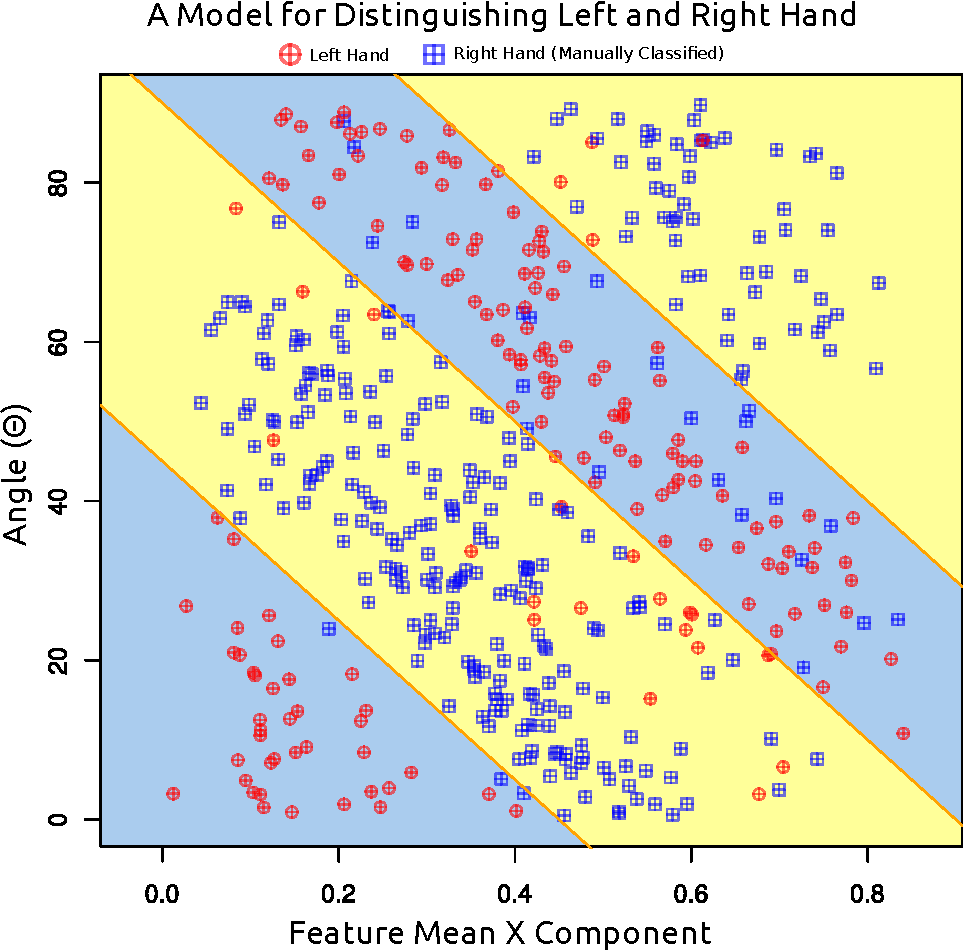
\includegraphics[type=pdf,ext=.pdf,read=.pdf,width=5in]{./img/hand_side_model}
\caption[A method for distinguishing hand side at the time grab or release actions are identified.]{
A method for distinguishing hand side at the time grab or release actions are identified. 
Red and blue markers represent actions that have been manually coded as left and right hand respectively, by a human observer after the study.
$\Theta$ is the angle of minimum enclosing rectangle just before the action was registered by the system.
The two regions shaded in blue represent the area classified as left hand by the model, while the region shaded in yellow represents the area that would be classified by the model as right hand.  
88\% of the points tested were classified correctly. 
}
\label{fig:hand.side.model}
\end{figure} 

\section{Post Study Questionnaire Results}
At the end of study, I provided a brief background questionnaire to the users.
This questionnaire asked about fatigue, general acceptance of the actions, potential new actions, user interaction feedback, and general feedback.
Figure \ref{fig:bg.q.2} summarizes the responses from participants to the multiple choice question related to fatigue and figure \ref{fig:bg.q.1} shows users' interest in using grab and release actions.

\begin{figure}
 \centering
 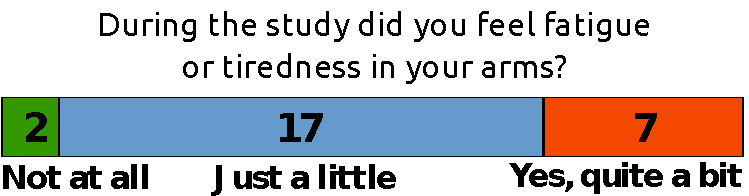
\includegraphics[type=pdf,ext=.pdf,read=.pdf,width=3in]{./img/bg.question.2}
 \caption{User feedback on how tired users felt after finishing the study.}
 \label{fig:bg.q.2}
\end{figure}

\begin{figure}
 \centering
 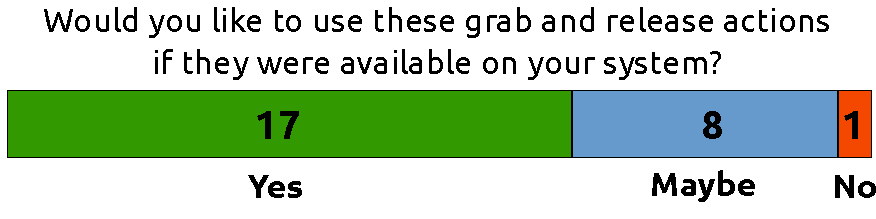
\includegraphics[type=pdf,ext=.pdf,read=.pdf,width=3in]{./img/bg.question.1}
 \caption{Users' interest in using grab and release action on their own computer systems.}
 \label{fig:bg.q.1}
\end{figure}

